\documentclass[a4paper]{article}
\usepackage[pdftex]{graphicx}
\usepackage[utf8]{inputenc}
\usepackage{enumerate}
\usepackage{siunitx}
\sisetup{locale=DE} 
\usepackage{icomma}
\usepackage{amssymb}
\usepackage{tikz}
\usepackage{href-ul}
\hypersetup{
	colorlinks=true,
	linkcolor=blue,
	urlcolor=blue}
\usepackage{geometry}
\geometry{a4paper, top=15mm, left=15mm, right=15mm, bottom=15mm,
	headsep=10mm, footskip=12mm}

\begin{document}
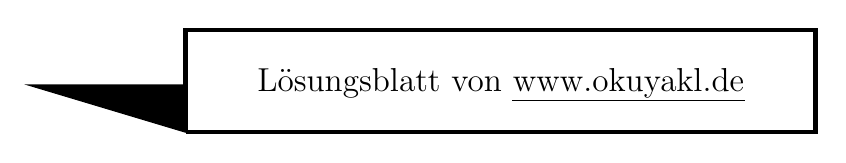
\begin{tikzpicture}(10,3)
	\draw[ultra thick](2,0) --(10,0) -- (10,1.3) --(2,1.3) -- (2,0);
	\draw[fill=black](2,0)-- (0,.6) -- (2,.6) -- (2,0);
	\node at (6,.6) {\large Lösungsblatt von \href{https://www.okuyakl.de}{www.okuyakl.de}};
\end{tikzpicture}
\vspace{0.5 cm}


\noindent{\bf Aufgabe 1. a)}\\
Jeder Körper besitzt eine Masse. Diese ist unveränderlich und bleibt gleich, egal ob  der Körper sich z.B. auf dem Mond oder auf der Erde befindet. Mit Gewicht hängt die Gewichtskraft zusammen, sie ist eine Größe, die man erhält, wenn man die Masse eines Körpers mit dem Ortsfaktor $g$ oder Gravitationsbeschleunigung multipliziert. Somit wiegt ein Körper mit einer bestimmten Masse auf der Erde mehr als auf dem Mond.
\vspace{0.5 cm}

\noindent{\bf Aufgabe 1. b)}\\
Auf die Feder wirkt die Kraft:
$$F_F = D \cdot s = \SI{24}{\newton\over \meter} \cdot \SI{0,13}{\meter} = \SI{3,12}{\newton} \approx \SI{3,1}{\newton}$$ 
Der Ortsfaktor des Planeten ist:
$$g_P = {F_F \over m} = {\SI{3,1}{\newton} \over \SI{0,15}{\kilogram}}= \SI{20,8}{\meter\over \second^2}$$
\vspace{0.5 cm}

\noindent{\bf Aufgabe 2.}\\
Die Masse des Würfels ist (wir dürfen hier mit Zentimetern und  Gramm rechnen):
$$ m= \varrho \cdot V = \SI{2,7}{\gram\over \centi\meter^3}\cdot (\SI{4,5}{\centi\meter})^3 = \SI{246}{\gram}$$
Seine Gewichtskraft ist gleich der Federkraft und damit ist die Dehnung $s$:
$$D \cdot s = m \cdot g \quad \Rightarrow \quad s = {m \cdot g \over D}= {\SI{0,25}{\kilogram} \cdot \SI{9,81}{\meter\over \second^2} \over \SI{90}{\newton\over\meter}} = \SI{0,027}{\meter}$$
Die ursprüngliche Federlänge ist:
$$l_0 = l - s =\SI{36,0}{\centi\meter} -\SI{2,7}{\centi\meter} = \SI{33,3}{\centi\meter}$$ 
\vspace{0.5 cm}

\noindent {\bf Aufgabe 3. a)}\\
Das Gesetz von Hooke besagt, dass die Federkraft proportional zur Ausdehnung (=Weg) ist. Um dies zu untersuchen befestigen wir die Feder, hängen verschiedene Gewichte mit der Gewichtskraft bis $\SI{12}{\newton}$  daran und notieren die Dehnung $s$. Die Wertepaare tragen wir in ein Diagramm ein. Wenn sie auf einer Ursprungsgeraden liegen, dann gilt für diese Feder das Hooke'sche Gesetz.   
\vspace{0.5 cm}

\noindent {\bf Aufgabe 3. b)}\\
Es gilt: 
$$F=D\cdot s \qquad \Leftrightarrow \qquad s={F \over D} \qquad (*)$$
Auf beide Federn wirkt die gleiche Kraft $F$, also dehnt sich Feder 1 der Härte $D_1$ um $s_1$ und Feder 2 der Härte $D_2$ um $s_2$. Die Gesamtdehnung ist $s_{ges}=s_1+s_2$:
$$s_{ges}=s_1+s_2= {F \over D_1}+ {F \over D_2} $$
mit eingesetzten Werten ergibt sich:
$$s_{ges}= {\SI{10}{\newton} \over\SI{250}{\newton\over \meter^2} }+{\SI{10}{\newton} \over \SI{500}{\newton\over \meter}}=\SI{0,060}{\meter}=\SI{6,0}{\centi\meter}$$
Für die Berechnung der Gesamtfederhärte gilt (*):
$$D_{ges}={F\over s_{ges}}={\SI{10}{\newton}\over \SI{0,060}{\meter}}=\SI{1,7e2}{\newton\over\meter}$$
\vspace{0.5 cm}

\newpage
\noindent{\bf Aufgabe 4.}\\
Die Dichte des Betons ist $\varrho=\SI{2,4}{\gram\over \centi\meter^3}=\SI{2,4}{\kilogram\over \deci\meter^3}$. Das Volumen in $\SI{}{\deci\meter^3}$ der Betonplatten ist:
$$V=(\SI{3}{\deci\meter})^2 \cdot \SI{0,5}{\deci\meter} \cdot 150 =\SI{675}{\deci\meter^3}$$
Dies entspricht einem Gewicht von:
$$m=\varrho \cdot V = \SI{2,4}{\kilo\gram\over \deci\meter^3} \cdot\SI{675}{\deci\meter^3} = \SI{1620}{\kilo\gram}$$
Er muss also dreimal fahren.
\vspace{0.5 cm}

\begin{center}
	\includegraphics[width=7 cm]{../../viecher/endcomic.pdf}
	
	Hier geht es zurück zum \href{https://www.okuyakl.de/phys/p8hukL405/aa405.pdf}{Aufgabenblatt}
\end{center}

\end{document}

